
\section{Experimentation}
\label{sec:experiments}
In this section, we aim to validate Scamplon by highlighting its properties and
compare them to the state-of-the-art random peer sampling protocols. In
particular, we inspect 3 properties characteristic of random graphs, namely the
\emph{average shortest path length}, the \emph{average clustering coefficient},
and \emph{the partial view size distribution}. Additionnaly, we investigate on
\emph{robusteness to random failures}.

Experiments are simulations ran on the well-known PeerSim simulator (REF). We
implemented Scamp, Cyclon, and Scamplon. The code is available on the Github
platform\footnote{http://github.com/anonymous4now}. Most of the experiments
involve 100, 1000, and 10000 peers.

\subsection{Clustering coefficient}
\begin{asparadesc}
\item[Objective:]
\item[Description:] The average clustering coefficient measures the
  connectivity of each peer's neighbourhood in the network.
  \begin{equation}
    \overline{C} = {1\over |\mathcal{N}|}\sum\limits_{x\in\mathcal{N}}C_x
    \end{equation}
    where $C_x$ is the local clustering coefficient of Peer $p_x$. The higher
    the coefficient, the more likely the network contains cliques. These
    experiments involve 100, 1000, and 10000 peers. Cyclon is set to be optimal
    at 1000 peers with $|\mathcal{P}|$ set to $7$. The exchanges concern $3$
    neighbours.
\item[Results:]
\item[Reasons:]
\end{asparadesc}

\begin{figure}
    \centering
    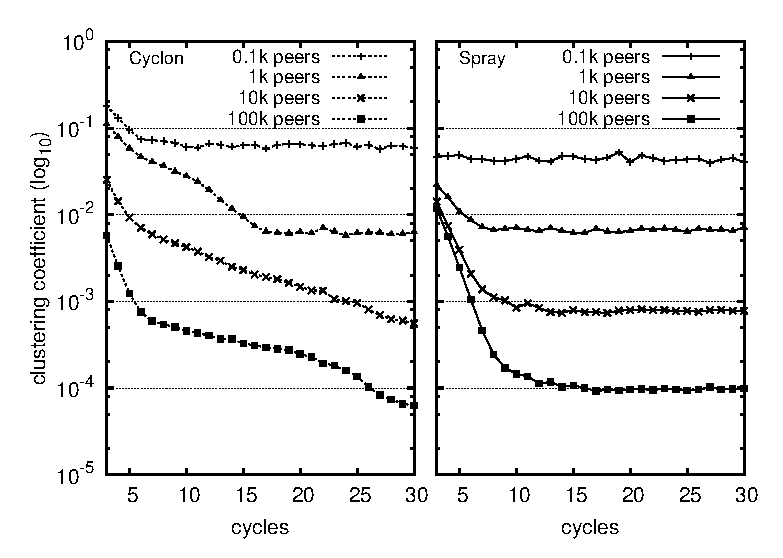
\includegraphics[width=0.49\textwidth]{img/cluster.eps}
    \caption{Clustering coefficient}
    \label{fig:clustering}
\end{figure}

\subsection{Average path length}
\begin{asparadesc}
\item[Objective:]
\item[Description:] The average path length is the average of the shortest path
  length between peers in the graph. It counts the minimum number of hops to
  reach a peer from another given peer. The lower the value, the faster a
  message can reach the whole network.
\item[Results:]
\item[Reasons:]
\end{asparadesc}


\subsection{Partial view size distribution}

\subsection{Resilience to failure}

\subsection{Churn}

\subsection{Synthesis}

%%% Local Variables:
%%% mode: latex
%%% TeX-master: "../paper"
%%% End:
